\documentclass{ximera}

%\addPrintStyle{..}

\begin{document}
	\author{Bart Lambregs}
	\xmtitle{Eenparige versnelde rechtlijnige beweging}{}
    \xmsource\xmuitleg




Een eendimensionale beweging waarvan de versnelling constant noemt  \textit{eenparig veranderlijke rechtlijnige be\-we\-ging} (EVRB). Eenparig betekent gelijkmatig; de snelheidsverandering is steeds gelijk. In symbolen: $a(t)=a$ waarbij $a$ een reëel getal is. Ook voor deze beweging kan je de plaatsfunctie en snelheidsfunctie bepalen en zo het verloop van de plaats en snelheid in functie van de tijd kennen. 

De versnelling is de afgeleide van de snelheid. Voor een constante versnelling is de snelheid in functie van de tijd een lineaire functie (in de tijd).\footnote{Strikt genomen zien we hier iets over het hoofd. A priori zou het immers kunnen dat er nog andere functies dan lineaire functies zijn waarvoor de afgeleide een constante functie is. Dat is echter niet het geval. Het bewijs hiervan zie je later dit jaar in het vak wiskunde. Je bewijst dat alle mogelijke functies die in aanmerking komen slechts op een constante na aan elkaar gelijk zijn.} Uit het snelheidsverloop kan je ook de plaats afleiden. De snelheid is de afgeleide van de plaatsfunctie. Voor een lineaire snelheidsfunctie is de positie dus een kwadratische functie (in de tijd). De afgeleide van een kwadratische functie is immers een lineaire functie.\footnote{Hier geldt een gelijkaardige opmerking als die in de vorige voetnoot.}

Dat de positie in functie van de tijd een tweedegraadsveeltermfunctie is, geeft in symbolen:\footnote{we gebruiken de constanten $p$, $q$ en $r$ i.p.v. $a$, $b$ en $c$ om verwarring met de betekenis van $a$ te voorkomen.}

\[
x(t)=pt^2+qt+r
\]

Aan de constanten $p$, $q$ en $r$ is deze formule kan een fysische betekenis gegeven worden. Dee snelheid is de afgeleide van deze plaatsfunctie en de versnelling komt overeen met de tweede afgeleide. Dit levert: 

\[
\begin{array}{rl}
v(t)&=\frac{dx}{dt}=2pt+q\\
a(t)&=\frac{d^2x}{dt^2}=2p%\nonumber
\end{array}
\]

Omdat de versnelling constant is, halen we uit de laatste regel dat $a(t)=a=2p\Leftrightarrow p=\frac{a}{2}$. Als we met $v_0$ de snelheid op tijdstip $t=0$ voorstellen ($v_0=v(0)$) en $t=0$ invullen, dan vinden we dat $q=v_0$. De constante $q$ stelt dus de beginsnelheid voor. Als we vervolgens met $x_0$ de positie op tijdstip $t=0$ voorstellen en $t=0$ invullen, dan vinden we dat $r=x_0$. De constante $r$ stelt dus de beginpositie voor.


\begin{theorem}
De plaatsfunctie $x(t)$ en de snelheidsfunctie $v(t)$ van een EVRB met versnelling $a$ worden gegeven door:
\[
\begin{array}{rcl}
x(t)&=&x_0+v_0t+\frac{1}{2}at^2\\
v(t)&=&v_0+at
\end{array}
\]
Hierin is $x_0$ de \textit{beginpositie} en $v_0$ de \textit{beginsnelheid}. Ze worden bepaald door de \textit{beginvoorwaarden} of \textit{randvoorwaarden}.
\end{theorem}	

Indien de beschrijving van de beweging niet op $t=0$ start maar op een gegeven tijdstip $t_0$, dan wordt in de beschrijving $t$ vervangen door $\Delta t= t-t_0$, de verstreken tijd vanaf het begintijdstip $t_0$. De plaatsfunctie en zijn afgeleide worden dan een klein beetje ingewikkelder:

\[
\begin{array}{rcl}
x(t)&=&x_0+v_0(t-t_0)+\frac{1}{2}a(t-t_0)^2\\
v(t)&=&v_0+a(t-t_0)
\end{array}
\]

Met de functies kan je de volgende formule voor de gemiddelde snelheid van een EVRB aantonen:%\footnote{Het formuletje is handig te gebruiken in veel vraagstukken door gebruik te maken van $\Delta x=\overline{v}\Delta t$.} 
\footnote{De afleiding van de gemiddelde snelheid is als volgt:
\begin{eqnarray*}
\overline{v}=\frac{\Delta x}{\Delta t}=\frac{x-x_0}{t-t_0}=\frac{v_0(t-t_0)+\frac{1}{2}a(t-t_0)^2}{(t-t_0)}=\frac{2v_0+a(t-t_0)}{2}=\frac{v_0+v}{2}.
\end{eqnarray*}}

\[
\overline{v}=\frac{v_0+v}{2}
\]

Blijkbaar houdt het eenparig toenemen van de snelheid in dat we het rekenkundig gemiddelde kunnen gebruiken voor de gemiddelde snelheid.



\begin{quickquestion*}{}{}
\begin{itemize}
	\item Op het moment\(t_1\) de snelheid gelijk aan nul, is de versnelling dan ook gelijk aan nul? 
	\item Op het moment\(t_1\) de vernelling gelijk aan nul, is de snelheid dan ook gelijk aan nul? 
	\item Als een auto vertraagd, is de versnelling dan negatief? 
\end{itemize}
\end{quickquestion*}

\begin{image}

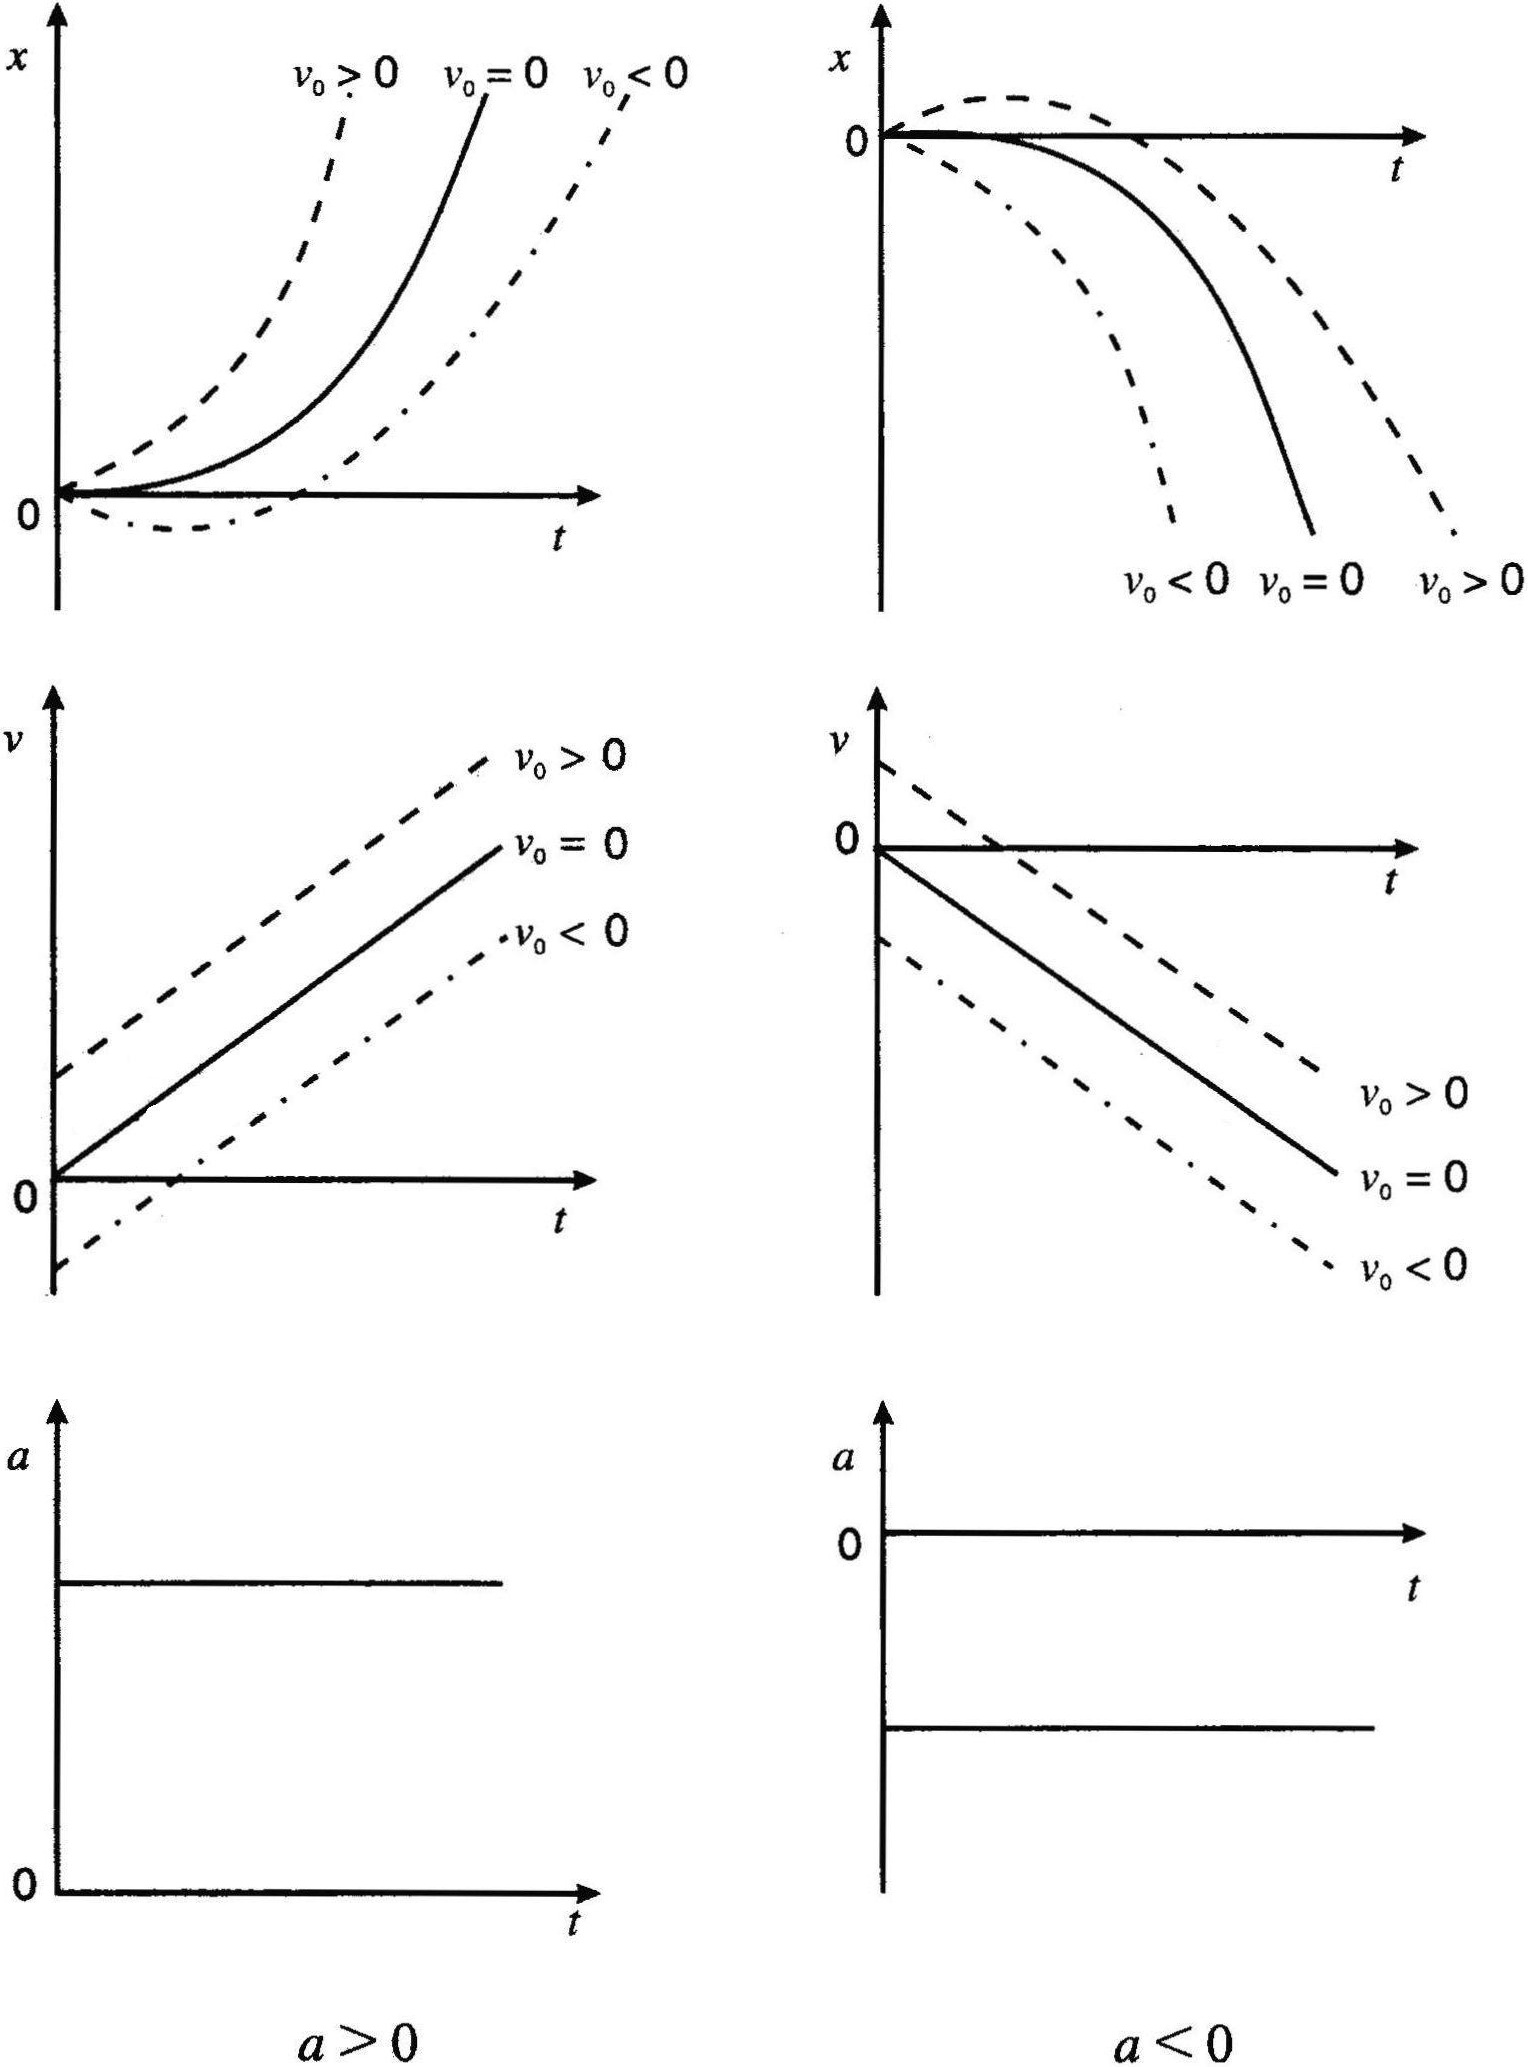
\includegraphics[width=\textwidth]{EVRB_grafieken}
%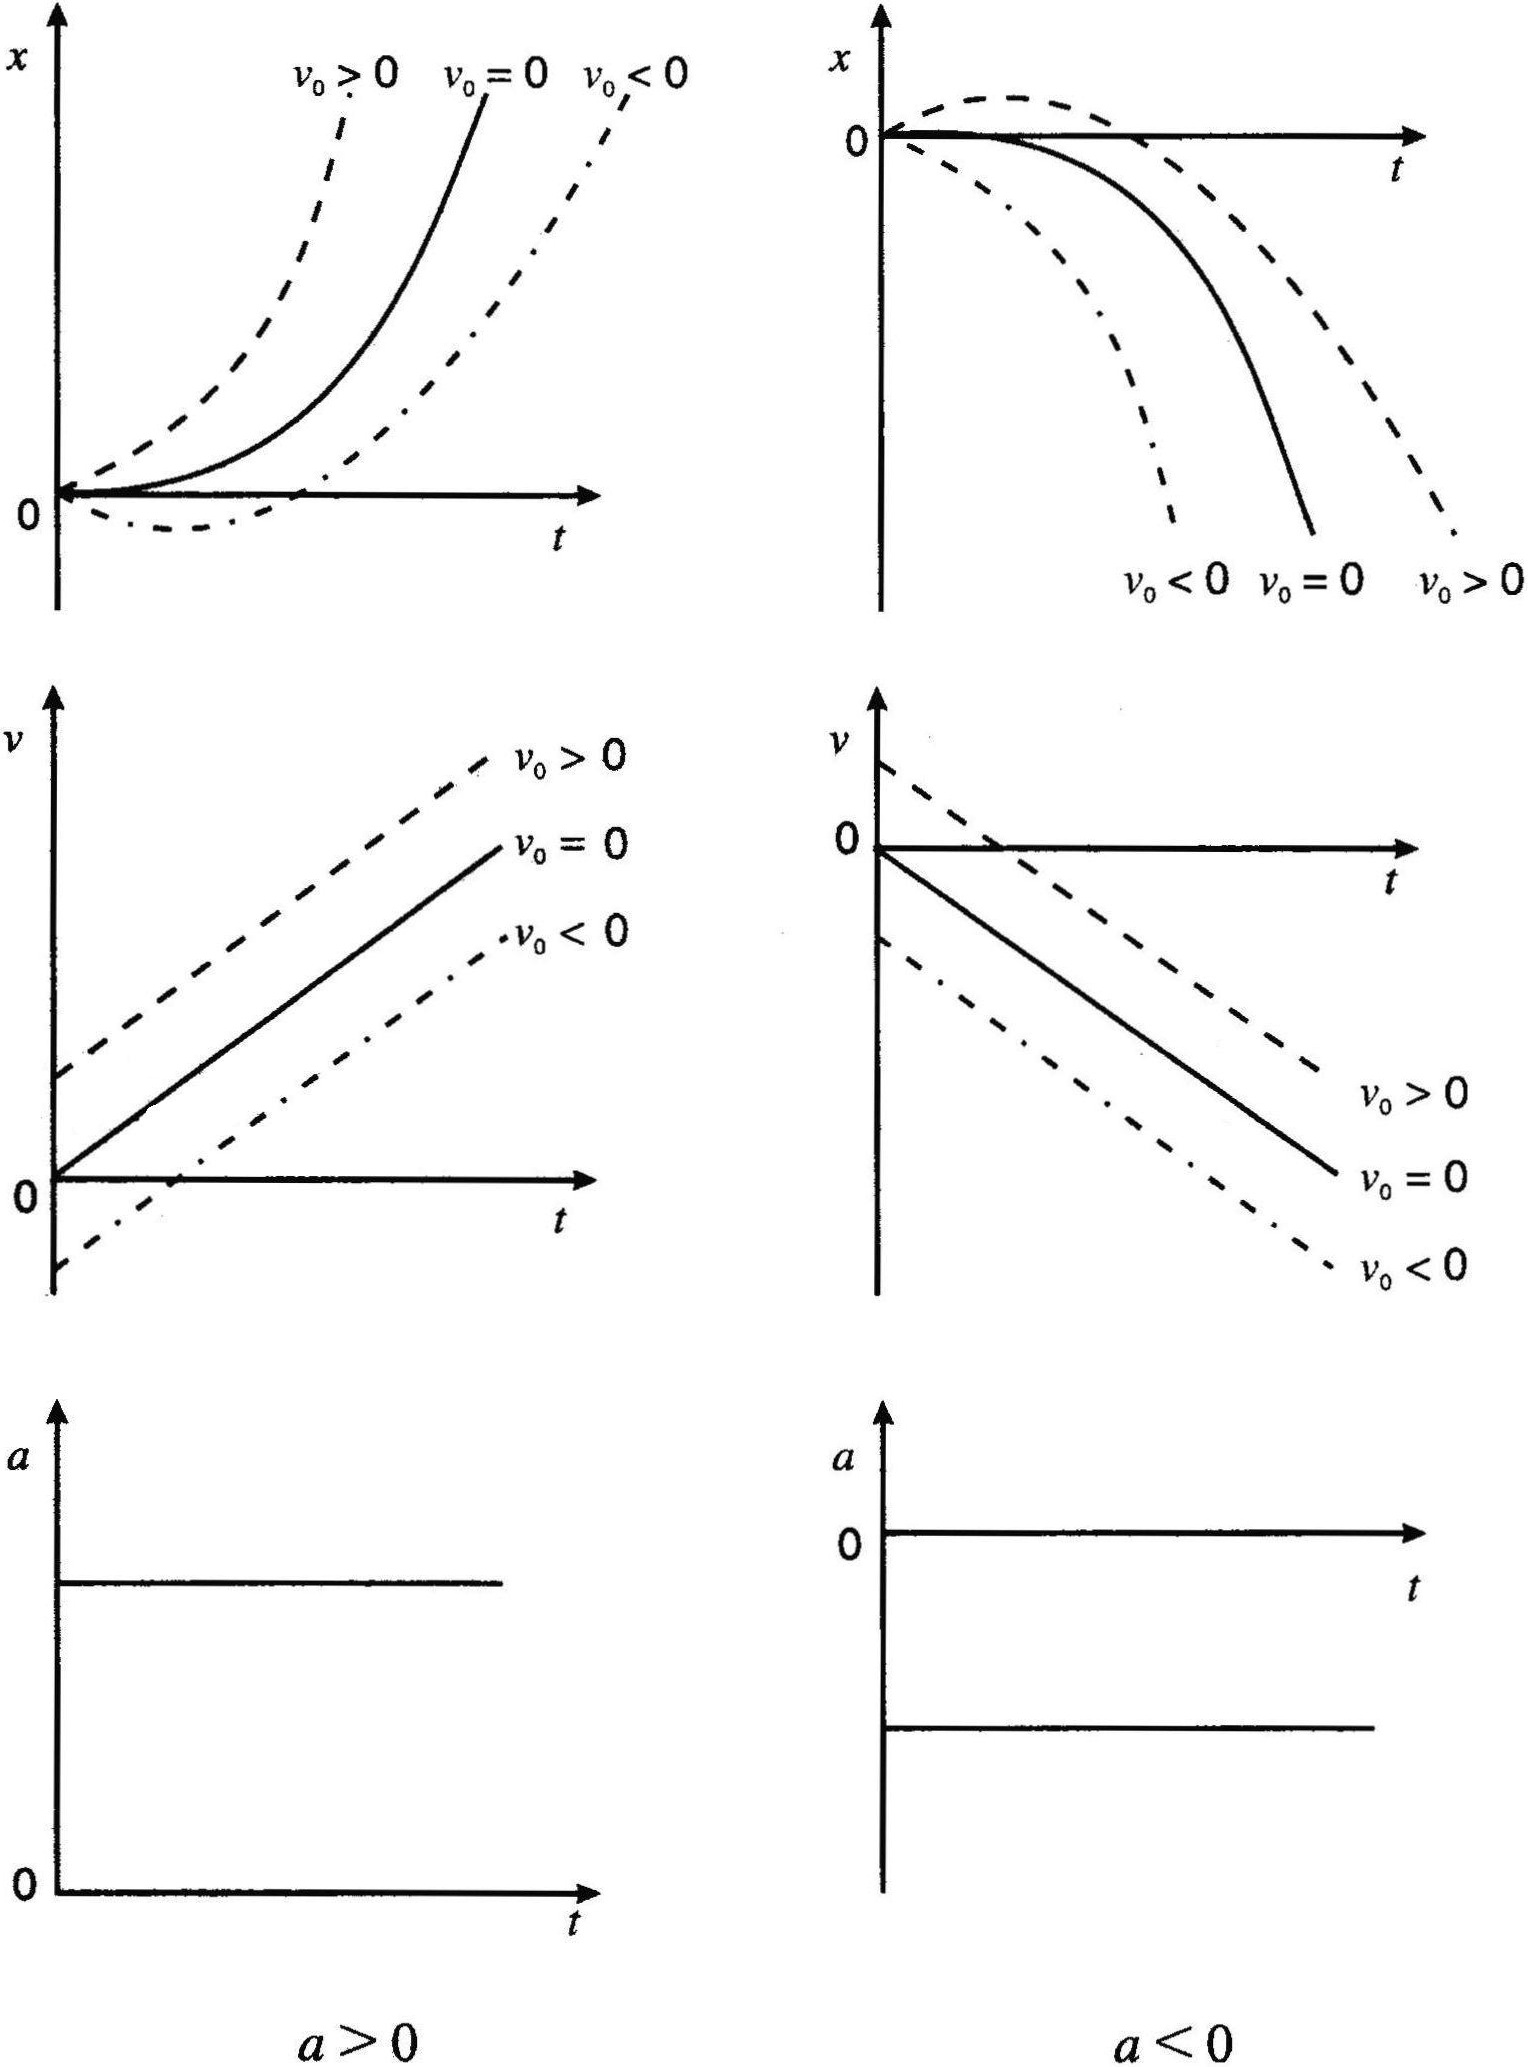
\includegraphics[height=\textheight]{EVRB_grafieken}
\end{image}
\captionof{figure}{Grafieken van een EVRB}




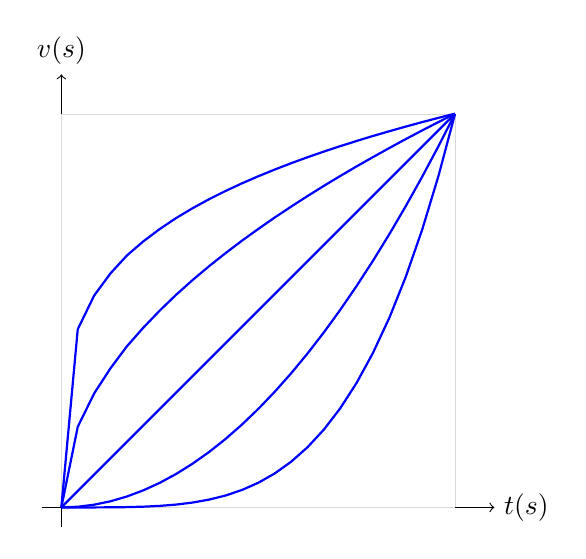
\begin{tikzpicture}[scale=5]
	% Axes
	\draw[->] (-0.05,0) -- (1.1,0) node[right] {$t(s)$};
	\draw[->] (0,-0.05) -- (0,1.1) node[above] {$v(s)$};
  
	% Grid lines (optional)
	\draw[very thin,color=gray!30] (0,0) grid (1,1);
  
	% Identity function
	\draw[thick,blue,domain=0:1] plot(\x,\x);
	\draw[thick,blue,domain=0:1] plot(\x,{pow(\x,2)});
	\draw[thick,blue,domain=0:1] plot(\x,{pow(\x,1/2)});
	% \draw[thick,red,domain=0:1] plot(\x,{pow(\x,3)});
	% \draw[thick,green,domain=0:1] plot(\x,{pow(\x,1/3)});
	\draw[thick,blue,domain=0:1] plot(\x,{pow(\x,4)});
	\draw[thick,blue,domain=0:1] plot(\x,{pow(\x,1/4)});
  

\end{tikzpicture}




\begin{exercise}

Een auto die $\SI{60}{km/h}$ rijdt, raakt een boom; de voorkant van de auto wordt in elkaar gedrukt en de bestuurder komt na $\SI{70}{cm}$ tot stilstand. Welke gemiddelde vertraging onderging de bestuurder tijdens de botsing? Druk je antwoord uit in $g$, waarbij $g=\SI{9,81}{m/s^2}$.
% \textit{Gegeven}  $v_0=\SI{16,7}{m/s}$%%%\newline$x=\SI{0,70}{m}$
% \textit{Gevraagd} $a$
% \textit{Oplossing} 
\begin{oplossing} 
Om de (constante) vertraging te vinden, hebben we de snelheidsverandering en de benodigde tijd nodig. De verandering in snelheid kennen we; de eindsnelheid van de auto moet nul worden maar de duur is niet onmiddellijk gegeven. Omdat de eindsnelheid nul is, kunnen we wel uit de snelheidsvergelijking van een eenparig veranderlijke beweging een \emph{uitdrukking} vinden voor die tijd die we vervolgens kunnen substitueren in de plaatsvergelijking. De enige onbekende is dan de gezochte versnelling.\footnote{M.b.v. de formule $\overline{v}=\frac{v_0+v}{2}$ voor de gemiddelde snelheid en de definitie voor de gemiddelde snelheid $\overline{v}=\frac{\Delta x}{\Delta t}$ is het antwoord sneller te vinden. Ga maar na \ldots}
%%%\newline
%%%\newline
Uit $v(t)=0$ of $0=v_0+at$ halen we een uitdrukking voor de tijd die nodig is om tot stilstand te komen:
\begin{align*}
t&=-\frac{v_0}{a}
\end{align*}
Substitutie van deze tijd in de plaatsfunctie levert:
\begin{align*}
x&=v_0t+\frac{1}{2}at^2\\
&=v_0\left(-\frac{v_0}{a}\right)+\frac{1}{2}a\left(-\frac{v_0}{a}\right)^2\\
%&=&-\frac{v_0^2}{a}+\frac{v_0^2}{2a}\\
&=-\frac{v_0^2}{2a}\\
\end{align*}
De versnelling is dan gelijk aan:
\begin{align*}
a&=-\frac{v_0^2}{2x}
\end{align*}
Invullen van de gegevens levert $a=\SI{-198}{m/s^2}$, wat gelijk is aan $20g$.
\end{oplossing}
\end{exercise}



	
	
\end{document}
